% !TEX root = ../main.tex

\chapter{Deterministic approach}
\label{chap:Deterministic approach}

\section{Modelling approaches}

Problem as defined in~\ref{chap:prob-def} can be reduced to two well known problems: transportation and min-cost max flow problem. In both cases knowning $\mathbf{x}$ implies all needed network parameters given $b, h > 0$.

\subsection{Transportation problem reduction}
\label{subs:Transportation problem reduction}

First we consider auxiliary variables $x'_{ij}$ which represent amount assigned from supply at time $i$ to demand at time $t$. This entails additional constraint:
\[x_i = \sum_j{x'_{ij}}\]

\begin{definition}{$\mathbf{C}$}
matrix defines cost for satisfying demand with specific raw supply material purchase date. It's element $c_{ij}$ equals:

\begin{equation*}
    c_{ij} = \begin{cases}
        b \left( i - j \right) + s_i & j < i \\
        h \left( j - i \right) + s_i & j \ge i
    \end{cases}
\end{equation*}
That is using purchaces raw materials at $i$ to satisfy demand at time moment $j$ incurs cost $c_{ij}$.
\end{definition}

Finally our original cost function~\ref{eq:cost-t} then equals to:

\begin{equation}
    \label{eq:cost-trans-t}
    c(t) = \sum_i{x'_{it}c_{it}}
\end{equation}

Under those modeling approaches optimal $x'_{ij}$ yields optimal $\mathbf{x}$

Transportation problem \autocite{or-textbook} is easy reduction since we have cost matrix $\mathbf{C}$ defining ``transportation'' costs associated with each possible assignment option. For successful reduction we only need adding dummy source or destination as described in \autocite{or-textbook}

%% min cost heuristic; fenwick tree\heap and other weird trickery to
%% compute it in O(n log n) time. It's overkill for this problem though

\subsection{Min cost max flow reduction}
\label{sub:Min cost max flow reduction}

We can exploit additional problem structure to achieve superior performance and modeling capabilities. In figure~\ref{fig:mcmf-model} we see network architecture.

\begin{figure}[h]
    \label{fig:mcmf-model}
    \centering
    
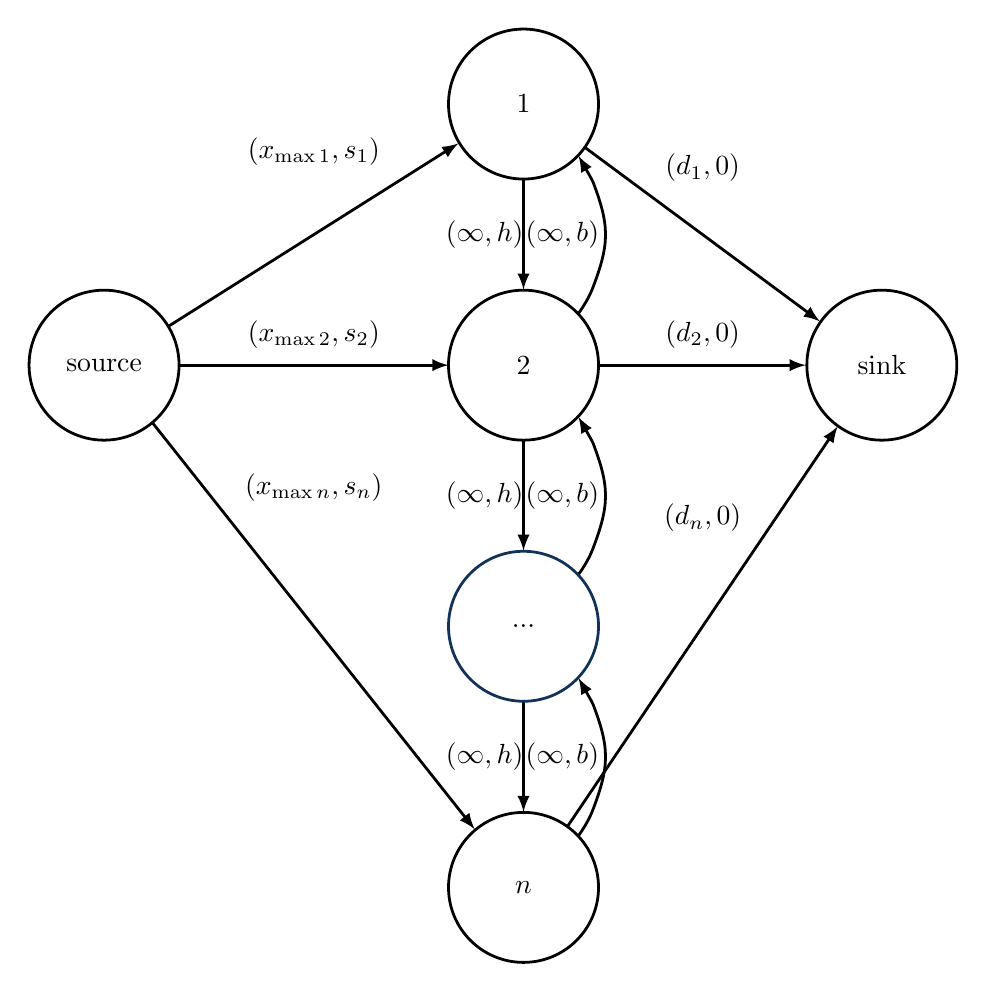
\begin{tikzpicture}[>=latex,line join=bevel,]
  \pgfsetlinewidth{1bp}
%%
\begin{scope}
  \pgfsetstrokecolor{black}
  \definecolor{strokecol}{rgb}{1.0,1.0,1.0};
  \pgfsetstrokecolor{strokecol}
  \definecolor{fillcol}{rgb}{1.0,1.0,1.0};
  \pgfsetfillcolor{fillcol}
  \filldraw (0.0bp,0.0bp) -- (0.0bp,336.0bp) -- (334.0bp,336.0bp) -- (334.0bp,0.0bp) -- cycle;
\end{scope}
\begin{scope}
  \pgfsetstrokecolor{black}
  \definecolor{strokecol}{rgb}{1.0,1.0,1.0};
  \pgfsetstrokecolor{strokecol}
  \definecolor{fillcol}{rgb}{1.0,1.0,1.0};
  \pgfsetfillcolor{fillcol}
  \filldraw (0.0bp,0.0bp) -- (0.0bp,336.0bp) -- (334.0bp,336.0bp) -- (334.0bp,0.0bp) -- cycle;
\end{scope}
  \pgfsetcolor{black}
  % Edge: n -> m
  \draw [->] (197.79bp,45.647bp) .. controls (199.91bp,48.565bp) and (201.75bp,51.712bp)  .. (203.0bp,55.0bp) .. controls (209.02bp,70.78bp) and (209.02bp,77.22bp)  .. (203.0bp,93.0bp) .. controls (202.92bp,93.205bp) and (202.84bp,93.41bp)  .. (197.79bp,102.35bp);
  \definecolor{strokecol}{rgb}{0.0,0.0,0.0};
  \pgfsetstrokecolor{strokecol}
  \draw (192.0bp,74.0bp) node {$(\infty, b)$};
  \draw (203.79bp,51.647bp) node {$$};
  \draw (203.79bp,96.353bp) node {$$};
  % Edge: m -> n
  \draw [->] (178.0bp,93.872bp) .. controls (178.0bp,84.622bp) and (178.0bp,74.113bp)  .. (178.0bp,54.189bp);
  \draw (164.0bp,74.0bp) node {$(\infty, h)$};
  \draw (184.0bp,90.872bp) node {$$};
  \draw (184.0bp,54.189bp) node {$$};
  % Edge: source -> 2
  \draw [->] (54.295bp,215.0bp) .. controls (78.339bp,215.0bp) and (114.12bp,215.0bp)  .. (150.97bp,215.0bp);
  \draw (102.5bp,226.0bp) node {$(x_{\max 2}, s_2)$};
  \draw (60.295bp,209.0bp) node {$$};
  \draw (144.97bp,209.0bp) node {$$};
  % Edge: 2 -> 1
  \draw [->] (197.79bp,233.65bp) .. controls (199.91bp,236.57bp) and (201.75bp,239.71bp)  .. (203.0bp,243.0bp) .. controls (209.02bp,258.78bp) and (209.02bp,265.22bp)  .. (203.0bp,281.0bp) .. controls (202.92bp,281.21bp) and (202.84bp,281.41bp)  .. (197.79bp,290.35bp);
  \draw (192.0bp,262.0bp) node {$(\infty, b)$};
  \draw (203.79bp,239.65bp) node {$$};
  \draw (191.79bp,284.35bp) node {$$};
  % Edge: n -> sink
  \draw [->] (193.82bp,48.934bp) .. controls (216.41bp,82.381bp) and (259.56bp,146.25bp)  .. (291.08bp,192.92bp);
  \draw (242.5bp,160.0bp) node {$(d_n, 0)$};
  \draw (187.82bp,42.934bp) node {$$};
  \draw (285.08bp,186.92bp) node {$$};
  % Edge: m -> 2
  \draw [->] (197.79bp,139.65bp) .. controls (199.91bp,142.57bp) and (201.75bp,145.71bp)  .. (203.0bp,149.0bp) .. controls (209.02bp,164.78bp) and (209.02bp,171.22bp)  .. (203.0bp,187.0bp) .. controls (202.92bp,187.21bp) and (202.84bp,187.41bp)  .. (197.79bp,196.35bp);
  \draw (192.0bp,168.0bp) node {$(\infty, b)$};
  \draw (203.79bp,145.65bp) node {$$};
  \draw (203.79bp,190.35bp) node {$$};
  % Edge: 2 -> m
  \draw [->] (178.0bp,187.87bp) .. controls (178.0bp,178.62bp) and (178.0bp,168.11bp)  .. (178.0bp,148.19bp);
  \draw (164.0bp,168.0bp) node {$(\infty, h)$};
  \draw (184.0bp,184.87bp) node {$$};
  \draw (184.0bp,148.19bp) node {$$};
  % Edge: 1 -> sink
  \draw [->] (200.26bp,293.27bp) .. controls (221.14bp,277.81bp) and (253.17bp,254.1bp)  .. (284.67bp,230.78bp);
  \draw (242.5bp,286.0bp) node {$(d_1, 0)$};
  \draw (206.26bp,287.27bp) node {$$};
  \draw (278.67bp,224.78bp) node {$$};
  % Edge: 1 -> 2
  \draw [->] (178.0bp,281.87bp) .. controls (178.0bp,272.62bp) and (178.0bp,262.11bp)  .. (178.0bp,242.19bp);
  \draw (164.0bp,262.0bp) node {$(\infty, h)$};
  \draw (184.0bp,281.87bp) node {$$};
  \draw (184.0bp,245.19bp) node {$$};
  % Edge: source -> n
  \draw [->] (44.515bp,194.16bp) .. controls (71.142bp,160.57bp) and (123.63bp,94.338bp)  .. (160.41bp,47.931bp);
  \draw (102.5bp,171.0bp) node {$(x_{\max n}, s_n)$};
  \draw (50.515bp,188.16bp) node {$$};
  \draw (154.41bp,53.931bp) node {$$};
  % Edge: source -> 1
  \draw [->] (50.307bp,229.07bp) .. controls (75.653bp,245.06bp) and (117.2bp,271.27bp)  .. (154.54bp,294.83bp);
  \draw (102.5bp,292.0bp) node {$(x_{\max 1}, s_1)$};
  \draw (56.307bp,223.07bp) node {$$};
  \draw (148.54bp,288.83bp) node {$$};
  % Edge: 2 -> sink
  \draw [->] (205.01bp,215.0bp) .. controls (223.63bp,215.0bp) and (248.96bp,215.0bp)  .. (279.59bp,215.0bp);
  \draw (242.5bp,226.0bp) node {$(d_2, 0)$};
  \draw (211.01bp,209.0bp) node {$$};
  \draw (273.59bp,209.0bp) node {$$};
  % Node: m
\begin{scope}
  \definecolor{strokecol}{rgb}{0.07,0.2,0.34};
  \pgfsetstrokecolor{strokecol}
  \draw (178.0bp,121.0bp) ellipse (27.0bp and 27.0bp);
  \definecolor{strokecol}{rgb}{0.0,0.0,0.0};
  \pgfsetstrokecolor{strokecol}
  \draw (178.0bp,121.0bp) node {$...$};
\end{scope}
  % Node: n
\begin{scope}
  \definecolor{strokecol}{rgb}{0.0,0.0,0.0};
  \pgfsetstrokecolor{strokecol}
  \draw (178.0bp,27.0bp) ellipse (27.0bp and 27.0bp);
  \draw (178.0bp,27.0bp) node {$n$};
\end{scope}
  % Node: 1
\begin{scope}
  \definecolor{strokecol}{rgb}{0.0,0.0,0.0};
  \pgfsetstrokecolor{strokecol}
  \draw (178.0bp,309.0bp) ellipse (27.0bp and 27.0bp);
  \draw (178.0bp,309.0bp) node {$1$};
\end{scope}
  % Node: source
\begin{scope}
  \definecolor{strokecol}{rgb}{0.0,0.0,0.0};
  \pgfsetstrokecolor{strokecol}
  \draw (27.0bp,215.0bp) ellipse (27.0bp and 27.0bp);
  \draw (27.0bp,215.0bp) node {source};
\end{scope}
  % Node: 2
\begin{scope}
  \definecolor{strokecol}{rgb}{0.0,0.0,0.0};
  \pgfsetstrokecolor{strokecol}
  \draw (178.0bp,215.0bp) ellipse (27.0bp and 27.0bp);
  \draw (178.0bp,215.0bp) node {$2$};
\end{scope}
  % Node: sink
\begin{scope}
  \definecolor{strokecol}{rgb}{0.0,0.0,0.0};
  \pgfsetstrokecolor{strokecol}
  \draw (307.0bp,215.0bp) ellipse (27.0bp and 27.0bp);
  \draw (307.0bp,215.0bp) node {sink};
\end{scope}
%
\end{tikzpicture}


    \caption{min cost max flot model. Arcs are labeled (capacity, cost)}
\end{figure}

\subsection{Feasable solution heuristic}
\label{subs:Feasable solution heuristic}
Since this problem has special structure, not found in original transportation problem, this heuristic enables us to construct better initial feasible solution. We can solve relaxed problem where backlogging is forbidden in $\mathcal{O}(n \log{} n)$ using greedy approach:

\begin{verbatim}
    For each $d_i$ in order from 1 to $n$ do:
        While $d_i$ not satisfied:
            Find cheapest $x_k$ positive supply node and
            satisfy as much as possible
\end{verbatim}

By the end of this procedure we're going to satisfy all demand in optimal way in case it's possible to to do. Naive implementation results in $\mathcal{O}(n^2)$ runtime, however we can use priority queue, with heap backing implementation for $\mathcal{O}(n\log{}n)$ runtime.

This priority queue is sorted by costs and since all costs raise by constant amount between $d_i$ and $d_{i+1}$ we can keep it updated in $\mathcal{O}(1)$.

\section{Variants}
\label{sec:Variants}

Problem as defined previously could seem rather simplistic and not allowing useful extensions users might want, such as current storage amount and similar. In following few subsections most useful extensions are described.

\subsection{Starting storage capacity}
in case we have already certain number of product in stock we can easily embed that knowledge into model by adding new supplier/node as new decision variable $x_0$. It's maximum, $x_{\max0}$ is equal to starting storage capacity, and $c_{0j} = \left( j - 1 \right) h$

\subsection{Ending storage requirement}
\label{subs:Ending storage requirement}
For example we'd like to have some extra product in stock by the end of analysis, and it's quite easy to accommodate such requirement. Simple add to $d_n$ ending storage requirement, thus obtaining new $d_n$.

\subsection{Time Shifted ordering}
\label{subs:Time Shifted ordering}
If we order raw materials at $t$ they might arrive at later time moment $t+\Delta_t$. This can easily be modeled via variable substitution. For different $\Delta_t$ depending on the $t$ or multiple suppliers see subsection~\ref{subs:Multiple raw material suppliers}

\subsection{Multiple raw material suppliers}
\label{subs:Multiple raw material suppliers}
Adding new raw material suppliers with different costs cannot be done as per original model specification, however reduction to presented problems is straightforward.

\subsection{Allowing future backlogging}
\label{subs:Allowing future backlogging}
In model as described, time stops at time moment $n$, however, in realistic scenario we're looking at only short time snapshot of ongoing process. To allow such future purchases to backlog at previous times, we can extend the model with $m$ future moments:
\begin{align*}
    d_{n+i} &= 0  && \\
    x_{\max{n+i}} &= y_i  && \text{allowable backlogging from future supply purchases}\\
    \mathbf{C}  & && \text{as previously defined, simply extended} \\
    \mathbf{s} &&& \text{extended with future costs}
\end{align*}
for $i$ in $1, 2, \dotsc, m$
